\documentclass[12pt]{zjutthesis}

\zjutTitle
  {论文中文题目}
  {Title of Thesis}
\zjutAuthor
  {作者姓名}
  {Author English}
\zjutMentor
  {教师姓名}{教\quad 授}
  {Mentor English}{Prof.}
\zjutMajor{软件工程}
\zjutAcademic{工程硕士} % 工学硕(博)士;专硕:工程硕士
\zjutCultiviate{全日制专业学位硕士} % 全日制专业学位硕士/全日制学术型硕(博)士
\zjutCollege{计算机科学与技术学院}

\zjutDate{2022}{06}    % 夏季06 春季01

\begin{document}
%%%%%%%% 封面 %%%%%%%%
\zjutpreface
%%%%%%%% 中文摘要 %%%%%%%%
\pagenumbering{Roman} % 摘要页码为大写罗马数字

\begin{AbstractCn}
  摘要的第一段主要阐述选题的意义。

  第二段简单介绍研究动机、方法、目的。从存在的问题出发,阐述你采用什
  么方法,依据什么理论来做什么事,从而解决了前面指出的那些问题及取得的成
  果。本文的主要工作和成果如下:

  1. 针对....采用...,提出了,,,,效果如何;

  2. 500 字左右;摘要应表达学位论文的中心内容,简短明了,摘取论文中
  的基本信息,体现科研工作的核心思想。内容包括本文的目的和意义、研究方法、
  研究成果、结论。主要介绍自己的工作和取得的成果。

  最后,对全文进行总结,对于工程硕士论文,可以强调下研究成果的实际运
  行效果。并对进一步的研究提出一些展望。

  \KeywordsCn{关键词数量为 4--6 个,每一关键词之间用逗号分开}
\end{AbstractCn}


%%%%%%%% 英文摘要 %%%%%%%%
\begin{AbstractEn}
  The graffiti period is the beginning of children's self-expression. Graffiti is a
  product of visual experience, body and finger muscle movement. It also reflects the
  child's physical and mental state. Therefore, Children's graffiti products are a hot issue
  in entertainment product.

  \KeywordsEn{Children's graffiti, deep learning, pool function, network transmission and communication, dynamic link library}
\end{AbstractEn}


%%%%%%%% 目录 %%%%%%%%
\frontmatter
\tableofcontents
\clearpage
\listoffigures
\listoffigureEng
\clearpage
\listoftables
\listoftableEng


%%%%%%%% 正文 %%%%%%%%
\mainmatter
\chapter{绪论}
\section{研究背景和意义}
绪论部分主要阐述论文选题的意义,说明研究的必要性、学术价值和实际意义,有具体项目背景的还说明项目来源[1]。
\section{研究目的}
\section{研究方案}
\section{预期目标}

\chapter{正文字体和公式用例}
\section{字体说明}
\begin{dinglist}{226}
  \item 一级标题,中文黑体三号,英文arial三号。居中,1.25倍行距,段前段后各0磅,上面空1行,下面空2行
  \item 二级标题,中文黑体四号,英文Times New Roman四号。两端对齐,1.25倍行距,段前24磅段后12磅
  \item 三级标题,中文黑体小四号,英文Times New Roman小四号。两端对齐,1.25倍行距,段前段后各0磅
  \item 正文,中文宋体小四号,英文Times New Roman小四号。两端对齐,首行缩进2字符,1.25倍行距,段前段后各0磅
\end{dinglist}

\section{公式例子}
\subsection{前向传播算法}
前向传播算法其过程都可以用如下公式表示:
\begin{equation}
  z^{i+1}=\sigma(a^{i+1})=\sigma(x^i\ast w^{i+1}+b^{i+1})
\end{equation}

其中,上标代表层数,星号$\ast$表示卷积操作,$b$表示偏置项,$\sigma$表示激活函数。
常见的激活函数如ReLu、Sigmoid、Tanh,详细在下一节中介绍。

\subsection{稀疏表示}
给定 $m$ 维特征向量 $X\in R^m$,它代表一段信号或是一副图片。
另外设定由基本组成元素构成的标准化基础矩阵 $D\in R^{m\times p}$,即字典 $D$,
它在信号中是不同频率的波形,在图像中则是构成图像的基本边和角。
$X$ 可以由矩阵 $D$ 中少量的列向量进行线性组合而得到,
其表示系数的矩阵为稀疏矩阵 $\alpha\in R^p$,如\autoref{eq:sparse}所示:

\begin{equation}
  X=D\alpha
  \label{eq:sparse}
\end{equation}

\chapter{图表规范和参考用例}
\section{表格规范和参考用例}
表格采用三线表,首末线1.5磅,第二线0.5磅,文字五号,单倍行距,行高0.7--0.8cm左右

\subsection{算法性能比较表格}

\begin{table}[htp]
  \centering
  \zihao{5}
  \bicaption
    {冰棒类训练数据集的实验均方误差MSE结果}
    {Experimental mean square error (MSE) of Popsicle training data set}
  \begin{tabular*}{0.8\hsize}{@{\extracolsep{\fill}}c c c}
    \toprule
    训练方法 & 训练集 & 测试集 \\
    \midrule
    Alexnet       & 0.261970 & 0.405175 \\
    VGG           & 0.310475 & 0.501455 \\
    Inception-BN  & 0.141686 & 0.285636 \\
    Resnet        & 0.079299 & 0.232052 \\
    \bottomrule
  \end{tabular*}
\end{table}

\begin{table}[htp]
  \centering
  \zihao{5}
  \bicaption
    {剑龙类训练数据集的实验均方误差MSE结果}
    {Experimental mean square error (MSE) of stegosaurus training dataset}
  \begin{tabular*}{0.8\hsize}{@{\extracolsep{\fill}}c c c}
    \toprule
    训练方法       & 训练集    & 测试集 \\
    \midrule
    Alexnet       & 0.371169 & 0.600909 \\
    VGG           & 0.203165 & 0.545861 \\
    Inception-BN  & 0.200882 & 0.589387 \\
    Resnet        & 0.128030 & 0.528496 \\
    \bottomrule
  \end{tabular*}
\end{table}

\subsection{系统目录规划表格}
\begin{table}[htp]
  \centering
  \zihao{5}
  \bicaption
    {系统目录规划表}
    {System directory planning table}
  \begin{tabular}{m{4cm}m{8cm}}
    \toprule
    目录                              & 名称及说明                                 \\
    \midrule
    /Doodle                         & 总目录,在此目录下存放系统的所有文件和目录                 \\
    /Doodle/ChangeTheme             & 用于存放更改系统主题显示的程序及相应的XML配置表             \\
    /Doodle/ChargeServer            & 用于存放系统收费程序及相应的XML配置表                  \\
    /Doodle/client                  & 用于存放系统客户端不同的主题程序及相应的XML配置表、DLL文件和图片资源 \\
    /Doodle/server                  & 用于存放系统服务器不同的主题程序及相应的XML配置表、DLL文件和动画资源 \\
    /Doodle/server/theme/data/score & 用于存放深度模型和评分程序、DLL及动画资源等相关文件           \\
    /Doodle/httphelper              & 用于存放系统通信程序                            \\
    /Doodle/CopyData                & 用于存放系统拷贝涂鸦数据程序                        \\
    /Doodle/dataserver              & 用于存放系统打印和分享程序及相应的XML配置表和相关文件          \\
    /Doodle/DeleterFiles            & 用于存放清除系统垃圾文件程序                        \\
    /Doodle/jiami                   & 用于存放系统加密程序                            \\
    \bottomrule
  \end{tabular}
\end{table}

\subsection{系统总体设计}

\begin{table}[htp]
  \centering
  \zihao{5}
  \bicaption
    {涂鸦系统总体类结构}
    {General class structure of graffiti system}
  \begin{tabular}{@{}|l|l|l|@{}}
    \hline
    模块名称                   & 类文件名称                   & 类文件名称                                                                                                       \\ \hline
    \multirow{2}{*}{全局配置类} & Configs.cs              & \begin{tabular}[c]{@{}l@{}}1 客户端服务器标志配置\\ 2 音效文件路径配置\\ 3 客户端和服务器网络传输方法名配置\\ 4 场景角色选择配置\end{tabular}         \\ \cline{2-3}
                           & GlobalContext.cs        & \begin{tabular}[c]{@{}l@{}}1 网络通信\\ 2 屏幕适应\end{tabular}                                                     \\ \hline
    \multirow{2}{*}{数据管理类} & JsonHelper.cs           & 数据管理,json 数据解析                                                                                              \\ \cline{2-3}
                           & ExcelHelpr.cs           & 数据管理,excel 数据解析                                                                                             \\ \hline
    画笔类                    & PensButtonController.cs & \begin{tabular}[c]{@{}l@{}}1 不同颜色的画笔管理和展示类\\ 2 切换画笔和画笔动画\end{tabular}                                       \\ \hline
    图像合成类                  & Drawing.cs              & \begin{tabular}[c]{@{}l@{}}1 将涂鸦用到的四张图片进行合成\\ 2 对服务器端接收到的图片进行裁切成\\ spine 动画需要的图片\end{tabular}               \\ \hline
    \multirow{3}{*}{图像合成类} & SindraxNetWorkClient.cs & \begin{tabular}[c]{@{}l@{}}局域网,网络通信客户端,直接绑定在摄\\ 像机上,定义客户端和服务器使用的\\ udp 传输数据的客户端方法\end{tabular}              \\ \cline{2-3}
                           & SindraxNetWorkServer.cs & \begin{tabular}[c]{@{}l@{}}1 网络通信服务端,启动 network,等待\\ 连接客户端,\\ 2 定义客户端和服务器使用的 udp 传输\\ 数据的服务端方法\end{tabular} \\ \cline{2-3}
                           & HttpHelper.cs           & 通过网络下载字符串                                                                                                   \\ \hline
    图像打分集成类                & scoreforimage.cs        & C\#调用 exe 程序,返回输出的分数                                                                                        \\ \hline
  \end{tabular}
\end{table}

\subsection{关键类接口}
如果某个类特别重要,并且具有明显的技术难度。则可以通过表格的形式给出类结构和接口说明。

\begin{table}[htp]
  \centering
  \zihao{5}
  \bicaption
    {视频流处理类}
    {Class of video streaming}
  \begin{tabular}{|p{.97\textwidth}|}
    \hline
    类名称:CCameraDS                                                                                        \\
    功能: 采用 DirectShow 对视频流数据进行处理                                                                         \\
    \hline
    \begin{lstlisting}[language=C++]
class CCameraDS
{
private:
    int m_nWidth, m_nHeight; // 图像宽度和高度
    long m_nBufferSize;      // 图像缓冲区大小
    IplImage* m_pFrame;      // 当前数据帧

public:
    // 打开摄像头,nCamID 指定打开哪个摄像头,取值可以为 0,1,2,...
    // bDisplayProperties 指示是否自动弹出摄像头属性页
    // nWidth 和 nHeight 设置的摄像头的宽和高,
    // 如果摄像头不支持所设定的宽度和高度,则返回 false
    bool OpenCamera(int nCamID, bool bDisplayProperties = true, int nWidth = 640, int nHeight = 480);

    // 关闭摄像头,析构函数会自动调用这个函数
    void CloseCamera();

    // 返回摄像头的数目
    // 可以不用创建 CCameraDS 实例,采用 int c=CCameraDS::CameraCount();得到结果。
    static int CameraCount();

    // 根据摄像头的编号返回摄像头的名字
    // nCamID: 摄像头编号
    // sName: 用于存放摄像头名字的数组
    // nBufferSize: sName 的大小
    // 可以不用创建 CCameraDS 实例,采用 CCameraDS::CameraName();得到结果。
    static int CameraName(int nCamID, char* sName, int nBufferSize);

    // 返回图像数据的为 RGB 模式的 Top-down (第一个字节为左上角像素)
    // 即 IplImage::origin = 0(IPL_ORIGIN_TL)
    IplImage* QueryFrame();
};
    \end{lstlisting} \\
    \hline
  \end{tabular}
\end{table}


\section{图规范和参考用例}
图宽度 10cm 左右,图内一般用英文标注,Arial 字体,
曲线粗细 1-2 磅中英文标题,中文宋体五号加粗,
英文 Times New Roman 五号加粗。
居中,1.25 倍行距,段前段后咯 0 磅,下面空一行

\subsection{功能架构图}
\autoref{fig:module}展示了系统主要功能模块设计图。

\begin{figure}[htp]
  \centering
  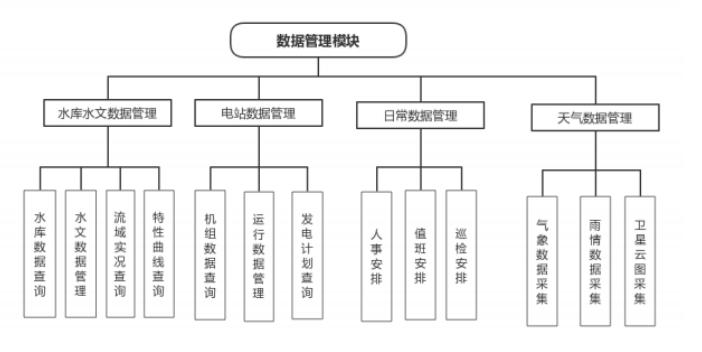
\includegraphics[width=\textwidth]{module}
  \bicaption
    {系统功能模块图}
    {System function module diagram}
  \label{fig:module}
\end{figure}

\subsection{系统架构图}
\autoref{fig:deploy}展示了系统架构图。

\begin{figure}[htp]
  \centering
  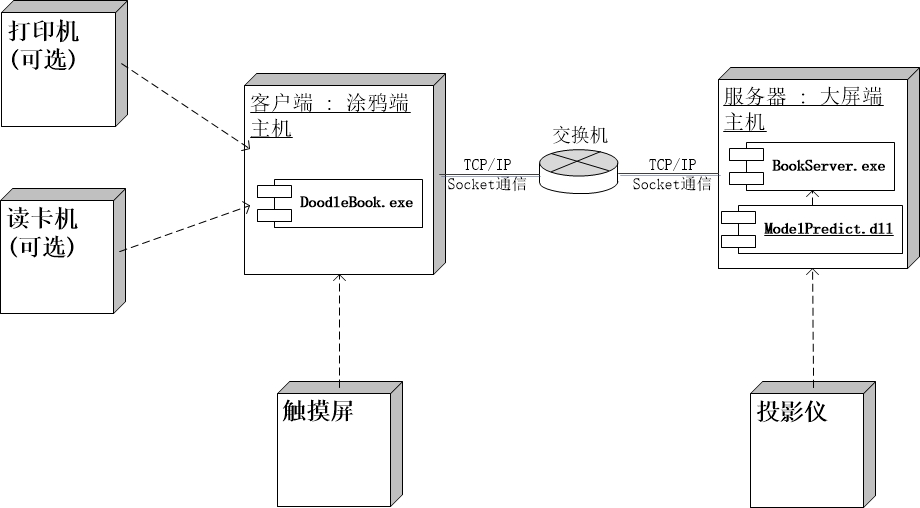
\includegraphics[width=0.6\textwidth]{deploy}
  \bicaption
    {儿童交互涂鸦系统部署图}
    {Deployment diagram of interactive graffiti system for children}
  \label{fig:deploy}
\end{figure}

\subsection{系统用例图}
\autoref{fig:usecase}展示了系统用例图。

\begin{figure}[!htp]
  \centering
  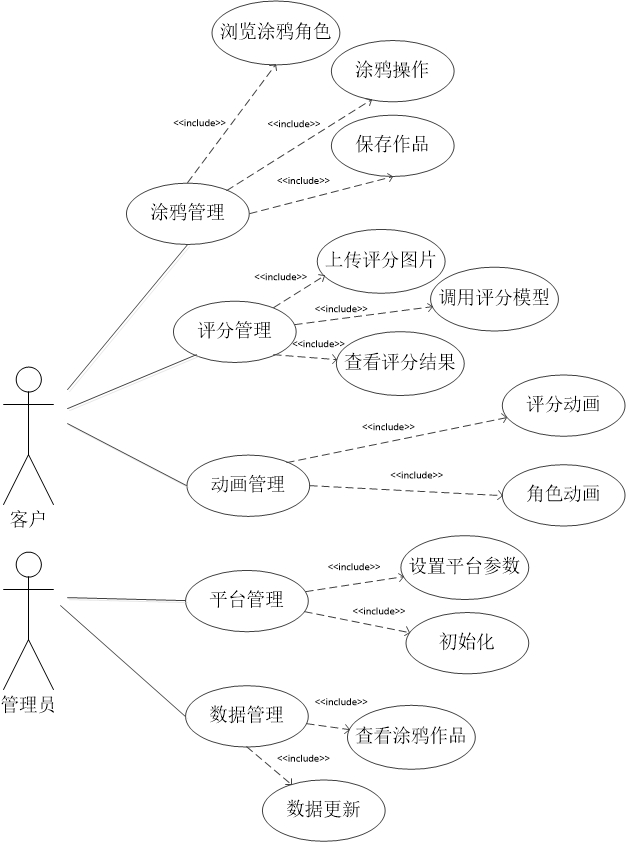
\includegraphics[width=0.6\textwidth]{usecase}
  \bicaption
    {系统用例图}
    {System use case diagrams}
  \label{fig:usecase}
\end{figure}

\subsection{算法流程图}
\autoref{fig:algo}展示了算法流程图。

\begin{figure}[!htp]
  \centering
  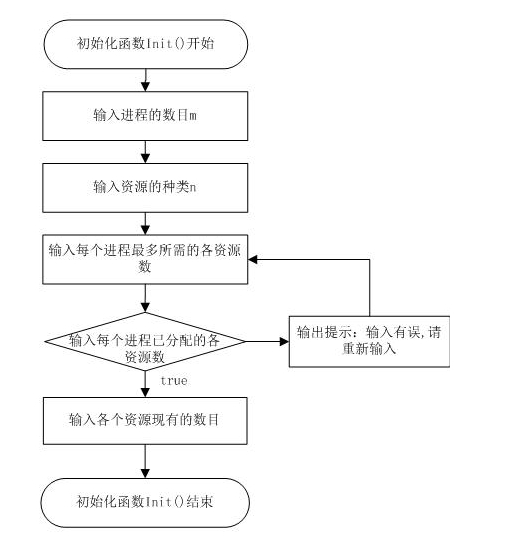
\includegraphics[width=0.6\textwidth]{algo}
  \bicaption
    {算法流程图}
    {The flowchart of the algorithm}
  \label{fig:algo}
\end{figure}

\subsection{数据库设计图}
\autoref{fig:database}展示了数据库设计图。

\begin{figure}[!htp]
  \centering
  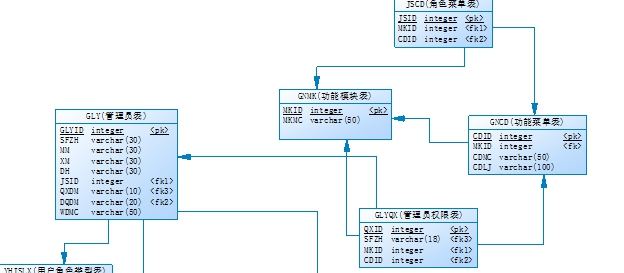
\includegraphics[width=0.6\textwidth]{database}
  \bicaption
    {系统的数据库设计}
    {The database designing of system}
  \label{fig:database}
\end{figure}

\subsection{算法性能分析图}
\autoref{fig:analysis}展示了算法性能分析图。

\begin{figure}[!htp]
  \centering
  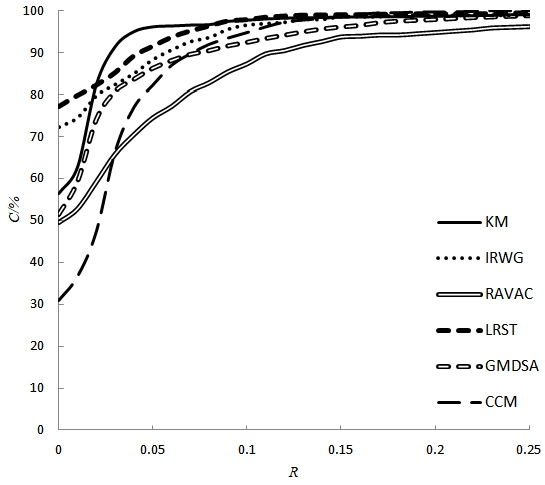
\includegraphics[width=0.6\textwidth]{analysis}
  \bicaption
    {DFAUST 数据库各算法定量分析}
    {Quantitative analysis of DFAUST database}
  \label{fig:analysis}
\end{figure}

\chapter{参考文献和参考用例}

参考文献应按文中引用出现的顺序列全,附于文末。
学位论文中列出的参考文献必须实事求是,论文中引用的必须列出,没引用的一律删去。

参考文献字体用5号,中文用宋体,英文用Times New Roman,行间距选1.4倍。

根据GB 3469 规定,以单字母方式标识各种参考文献类型:

\begin{table}[htp]
  \centering
  \resizebox{\linewidth}{!}{
  \begin{tabular}{ccccccccccc}
    \toprule
    参考文献类型 & 专著 & 论文集 & 析出论文 & 报纸文章 & 期刊文章 & 学位论文 & 报告 & 标准 & 专利 & 其他文献 \\
    \midrule
    文献类型标识 & M & C & A & N & J & D & R & S & P & Z \\
    \bottomrule
  \end{tabular}
  }
\end{table}

对于数据库,计算机程序及光盘图书等电子文献类型的参考文献,以下列字母为标识:
\begin{table}[htp]
  \centering
  \begin{tabular}{cccc}
    \toprule
    \textbf{参考文献类型} & \textbf{文献类型标识} \\
    \midrule
    数据库(网上)         & DB (DB/OL)      \\
    计算机程序(磁盘)       & CP (CP/DK)      \\
    光盘图书            & M/CD            \\
    \bottomrule
  \end{tabular}
\end{table}

用到5类文献码,分别是[C](会议)、[J] (杂志)、[M](书籍)、[EB/OL](在线刊物)、[D](研究生论文)。注意:1)学术会议的文献标识码为[C],不是[A];2)不要出现太多的D和M,会让专家感觉研究不够深入;3) 一般参考文献50篇以上,要有中文和英文参考文献,而且英文参考文献要在20篇以上,否则专家会觉得对国内外研究现状不了解;4)中文参考文献中尽量不要出现低档次期刊(例如某某大学学报(普通高校的学报通常质量一般)、计算机工程与应用、计算机应用研究等),尽量引用高水平期刊(例如计算机学报、软件学报、计算机研究与发展、电子学报、电子与信息学报等)5)外国人名字按照该写法:Igarashi T;6)近5年的参考文献要占到1/3以上 7)参考文献不同类型写法;

1)会议写法:Tang K K, Song P, Chen X P. Signature of geometric centroids for 3D local shape description and partial shape matching[C], Proceedings of the Asian Conference on Computer Vision. Heidelberg: Springer, 2016, 10115: 311-326

2)杂志写法:Song C Z, Yuille A. Region competition: unifying snakes, region growing, and Bayes/MDL for multiband image segmentation[J]. IEEE Transactions on Pattern Analysis and Machine Intelligence, 1996, 18(9):884-900

3)论文写法:陈国栋. 基于代理模型的多目标优化方法及其在车身设计中的应用[D]. 湖南大学, 2012.

4)书籍写法:中国能源中长期发展战略研究项目组. 中国能源中长期 (2030、2050) 发展战略研究[M]. 科学出版社, 2011.

5)在线刊物写法:王明亮. 关于中国学术期刊标准化数据库系统工程的进展 [EB/OL]. http://www.cajcd.edu.cn/pub/wml.txt/980810-2.html,  1998-08-16

\section{测试引用}
测试引用:
\cite{zhangkun1994}
\cite{zhukezhen1973}
\cite{dupont1974bone}
\cite{zhengkaiqing1987}
\cite{jiangxizhou1980}
\cite{jianduju1994}
\cite{merkt1995rotational}
\cite{mellinger1996laser}
\cite{bixon1996dynamics}
\cite{mahui1995}
\cite{carlson1981two}
\cite{taylor1983scanning}
\cite{taylor1981study}
\cite{shimizu1983laser}
\cite{atkinson1982experimental}
\cite{kusch1975perturbations}
\cite{guangxi1993} \\
\cite{huosini1989guwu}
\cite{wangfuzhi1865songlun}
\cite{zhaoyaodong1998xinshidai}
\cite{biaozhunhua2002tushu}
\cite{chubanzhuanye2004}
\cite{who1970factors}
\cite{peebles2001probability}
\cite{baishunong1998zhiwu}
\cite{weinstein1974pathogenic}
\cite{hanjiren1985lun}
\cite{dizhi1936dizhi}
\cite{tushuguan1957tushuguanxue}
\cite{aaas1883science}
\cite{fugang2000fengsha}
\cite{xiaoyu2001chubanye}
\cite{oclc2000about}
\cite{scitor2000project}

\chapter{研究生论文专家评审常见问题及修改方案}
论文评审是对研究生毕业前的一道重要程序。
也是决定研究生能否顺利毕业的前提和关键。
每年都有研究生因为论文评审不通过无法正常毕业。
为了帮助研究生顺利通过论文评审。
在这里,我们汇总了评审过程中的一些常见问题以及相应的修改方案,
以帮助研究生顺利通过论文评审。

\section{专家评审要点}
\begin{enumerate}
  \item 选题有重要的理论意义或工程实用价值;
  \item 综述能够对已有研究进行全面总结和分析存在的问题; 解决研究问题的方案设计合理;
  \item 所提出的理论或方法上有创新性或者是技术方面有明显的突破;
  \item 工作量饱满,并且技术路线上有较高的实现难度;
  \item 论文写作条理清晰,分析严谨,图表规范、参考文献引用规范
\end{enumerate}
\section{专家评审典型意见及建议修改方案}
本节对于历年专家反馈回来的典型意见进行汇总并给出建议修改意见,供各位研究生在撰写论文时参考。
\subsection{中文摘要方面的问题}
专家意见:
1)摘要背景知识介绍过多,论文所取得的成果没有体现;
2)建议作者在突出创新点的基础上按目的、方法、结果和结论撰写摘要。

修改方案:摘要通常第一段写背景、意义。
从第二段开始写自己的工作。
需要体现作者本人的工作,未说明所完成工作的应用效果等
(成果例如该算法把识别准确率提高了???;该系统已经在???应用,减少了???。)。
同时需避免的一些常见问题:
书写时,注意要符合中文语法,做到语句通顺、言简意赅、一定要使用书面语言,去口语化,
例如:不要出现“我”或者 “我们”,“这个”用“该”代替,“也就是说”用“即”,
“它的功能”用“其功能”代替等等。
第一次出现缩写的地方给出全称,如:DBS(Database system,数据库系统)。

\chapter{结论与展望}
\section{结  论}
\linespread{1.5}
简要回顾所做的工作,包括为什么要做这件研究工作,
采用什么方法,做了哪些事,取得了哪些结果,
是否有实验、仿真或实际应用,效果如何?
对推进本学科发展有什么作用?
要注意不要完全复制摘要,既有类似之处,但也不完全相同。
\section{展  望}
可结合技术发展趋势,分析本文尚存在的问题,
简要说明下一步可如何做以解决这些存在的问题,
同时展望一下该方向的发展前景。

%%%%%% 参考文献 %%%%%%
\backmatter
\bibliography{bib.bib}


%%%%%% 致谢 %%%%%%
\chapter{致  谢}
时光如梭,岁月如歌,接到研究生入学通知书时的场景还历历在目,转瞬又将离开校园,一别经年。

%%%%%% 作者简介 %%%%%%
\chapter{作者简介}
\section{作者简历}
××××年××月出生于××××。

××××年××月——××××年××月,××大学××院(系)××专业学习,攻读××学硕士学位。

\section{攻读硕士学位期间发表的学术论文}
 [1]	Jia M M, Yi N N, Bing O, Ding P Q, Wu R.. Maximum spatial-temporal isometric cluster for dynamic surface correspondence, The Visual Computer, 2019, accepted. (SCI源期刊,IF = X.XX)

[2]	Jia M M, Yi N N, Bing O, Ding P Q. Article Title. Journal Title, 2015, 118(1/2): 389–398. (SCI收录,IDS号为XXXXX,IF= X.XX)

[3]	贾某某, 易某某, 邴某某, 等. 多视图卷积网络加权优化. 计算机辅助设计与图形学学报, 2018, xx(x): xx–xx. (EI收录号:2014XXXXXXXXX)

\section{参与的科研项目及获奖情况}
 [1]	易某某, 贾某某. ××××××××××, 国家自然科学基金项目. 编号: ××××.

[2]	易某某, 贾某某. ××××××××××××××××××. ××省科学技术一等奖, 2014.

\section{发明专利}
 [1]	贾某某. ××××××××××××. 中国, 2013 1 0513271.2 [P]. 2015-04-26.

%%%%%% 附录 %%%%%%
\chapter{学位论文数据集}
\end{document}
